\subsection{Kegelradpaar \hfill ME}

\begin{minipage}{0.45\linewidth}
        \begin{footnotesize}
            \begin{center}
            \begin{empheq}[box=\fbox]{align*}
                i &= \left\{...\right\} = \frac{d_{m2}}{d_{m1}}\\ &= \frac{d_{e2}}{d_{e1}} = \frac{sin(\delta_2)}{sin(\delta_1)}
            \end{empheq}
        \begin{scriptsize}
            $d_m$ = mittlerer Teilkreis-$\diameter$
            \\$R_m$ = mittlere Teilkegellänge
            \\$d_e$ = äusserer Teilkreis-$\diameter$
            \\$R_e$ = äussere Teilkegellänge
            \\$\Sigma$ = Achsenwinkel
            \\$\delta$ = Teilkegelwinkel
        \end{scriptsize}
        \end{center}
        \end{footnotesize}
\end{minipage}
\vspace{0.5mm}\begin{minipage}{0.53\linewidth}
    \begin{center}
        \frame{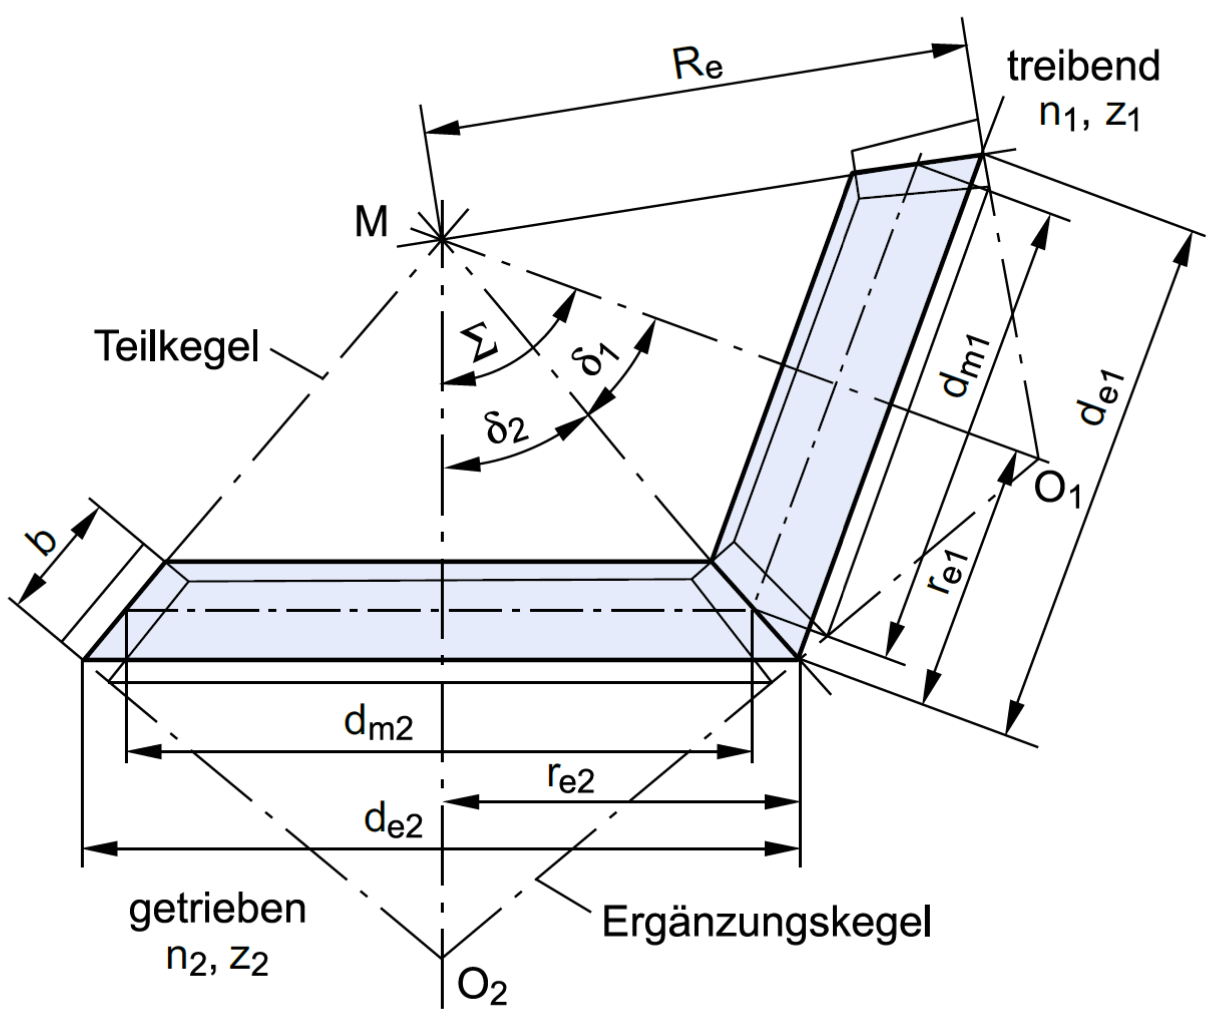
\includegraphics[width = 1.0\linewidth]{src/images/MAEIP_Kegelrad}}
    \end{center}
\end{minipage}
\cbreak
\begin{footnotesize}
    \begin{empheq}[box=\fbox]{align*}
    &\text{Für $\Sigma \leq 90^\circ$:} \qquad \qquad \qquad \qquad \text{Für $\Sigma > 90^\circ$:}
    \\&tan(\delta_1) = \frac{sin(\Sigma)}{i + cos(\Sigma)} \; \; \; \; \qquad tan(\delta_1) = \frac{sin(180^\circ - \Sigma)}{i - cos(180^\circ - \Sigma)}
    \end{empheq}
    \begin{empheq}[box=\fbox]{align*}
        \Sigma = \delta_1 + \delta_2
    \end{empheq}
    \\\textbf{Kegelrad-Differential:}
    \mathbox{
        M_{an} = 2 \cdot M_{ab}
    }
\end{footnotesize} 